% chapter02.tex

 %%%%%%%%%%%%%%%%%%%%%%%%%%%%%%%%%%%%%%%%%%%%%%%%%%%%%%%%%%%%%%%%%%%%%%%%%%%%%
 %                                                                           %
 %    PyMS documentation                                                     %
 %    Copyright (C) 2005-8 Vladimir Likic                                    %
 %                                                                           %
 %    The files in this directory provided under the Creative Commons        %
 %    Attribution-NonCommercial-NoDerivs 2.1 Australia license               %
 %    http://creativecommons.org/licenses/by-nc-nd/2.1/au/                   %
 %    See the file license.txt                                               %
 %                                                                           %
 %%%%%%%%%%%%%%%%%%%%%%%%%%%%%%%%%%%%%%%%%%%%%%%%%%%%%%%%%%%%%%%%%%%%%%%%%%%%%

\chapter{Using PyMS}

\section{Introduction}

This chapter demonstrates main functions of PyMS in a tutorial like manner.
The data files used in the examples are provided in the project 'pyms-data'.
The commands executed interactively are grouped together by example, and
provided as Python scripts in the project 'pyms-test'.

The setup used in the examples below is as follows. The projects 'pyms',
'pyms-test', 'pyms-docs', and 'pyms-data' were downloaded in the directory
{\tt /home/current/proj/PyMS}. In the project 'pyms-test' there is a directory
corresponding to each example coded with the example number (ie.
{\tt pyms-test/01/} corresponds to Example 1). In each example directory
there is a script named 'proc.py' which contains the commands given in
the example. Provided that the paths to 'pyms' and 'pyms-data' are set
properly, these scripts could be run by simply:

\$ python proc.py

Before running each example the Python interpreter was made aware of the
PyMS location with the following commands:

\begin{verbatim}
import sys
sys.path.append("/home/current/proj/PyMS/")
\end{verbatim}

For brevity these commands will not be shown in the examples below, but
they are included in 'pyms-test' example scripts.  The above path need
to be adjusted to match your own location of pyms.

All data files (raw data files, peak lists etc) used in the example below
can be found in 'pyms-data'.


\section{Example 1: Reading of GC-MS data and basic manipulation of
data}

\subsection{Reading ChemStation GC-MS data into PyMS}

\noindent
{\em This example is in pyms-test/01}

The PyMS package pyms.IO provides capabilities to read the raw GC-MS
data stored in the ANDI-MS format. The function IO.ANDI.ChemStation()
provides the interface to ANDI-MS data files saved from Agilent
ChemStation software.\footnote{ANDI-MS data format stands for Analytical
Data Interchange for Mass Spectrometry, and was developed for the
description of mass spectrometric data developed in 1994 by Analytical
Instrument Association. ANDI-MS is essentially a recommendation, and
it is up to individual vendors of mass spectrometry processing software
to implement "export to ANDI-MS" feature in their software.}

The file '0510\_217.CDF' is a GC-MS experiment exported from Agilent
ChemStation (located in 'pyms-data'). This file can be loaded in the
memory as follows:

\begin{verbatim}
>>> from pyms.IO.ANDI.Class import ChemStation
>>> andi_file = "/home/current/proj/PyMS/pyms-data/0510_217.CDF"
>>> andi_data = ChemStation(andi_file)
 -> Processing netCDF file '/home/current/proj/PyMS/pyms-data/0510_217.CDF'
    [ 2784 scans, masses from 50 to 550 ]
>>>
\end{verbatim}

\noindent
The above command creates the object 'andi\_data' which is an {\em instance}
of the class IO.ANDI.ChemStation.

\subsection{Exploring an ANDI-MS data object}

The object 'andi\_data' has several attributes and methods associated with it.

\begin{verbatim}
>>> print "ANDI-MS data filename:", andi_data.get_filename()
ANDI-MS data filename: /home/current/proj/PyMS/pyms-data/0510_217.CDF
\end{verbatim}

The method {\tt get\_tic()} return total ion chromatogram (TIC) of the data
as an IonChromatogram object:

\begin{verbatim}
tic = andi_data.get_tic()
\end{verbatim}

\noindent
An IonChromatogram object is a one dimensional vector containing
mass intensities as a function of retention time. This can can be either
m/z channel intensities (for example, ion chromatograms at m/z = 65),
or cumulative intensities over all measured m/z (TIC).

The method {\tt get\_ic\_at\_index(i)} returns i-th ion chromatogram, as
an IonChromatogram object. For example, to get the first ion chromatogram
from the data:

\begin{verbatim}
ic = andi_data.get_ic_at_index(1)
\end{verbatim}

The method {\tt get\_ic\_at\_mass(MZ)} returns the ion chromatogram for
m/z = MZ.  For example, to get the ion chromatogram that corresponds
to m/z = 73:

An ion chromatogram object has a method {\tt is\_tic()} which returns
True is the ion chromatogram is TIC, False otherwise:

\begin{verbatim}
>>> print "'tic' is a TIC:", tic.is_tic()
'tic' is a TIC: True
>>> print "'ic' is a TIC:",ic.is_tic()
'ic' is a TIC: False
\end{verbatim}

\subsection{Writing data to a file}

The method {\tt write()} of IonChromatogram object allows one to save
the ion chromatogram object to a file:

\begin{verbatim}
>>> tic.write("output/tic.dat", minutes=True)
>>> ic.write("output/ic.dat", minutes=True)
\end{verbatim}

\noindent
The flag minutes=True indicates that retention time will be saved in minutes.
The ion chromatogram object saved with with the {\tt write{}} method is a
plain ASCII file which contains a pair of (retention time, intensity) per
line:

\begin{verbatim}
$ head tic.dat
  5.0944      745997.0000
  5.1002      726566.0000
  5.1059      717704.0000
  5.1116      684214.0000
  5.1173      701866.0000
  5.1230      893306.0000
  5.1287     1278099.0000
  5.1345     1290984.0000
  5.1402      925558.0000
  5.1459      644122.0000
\end{verbatim}

\noindent
Figure \ref{tic-plot} shows the plot of the file 'tic.dat' produced with the
program Gnuplot. The Gnuplot script used to produce this plot is provided
as pyms-test/01/output/plot.gnu.

\begin{figure}[htp]
\begin{center}
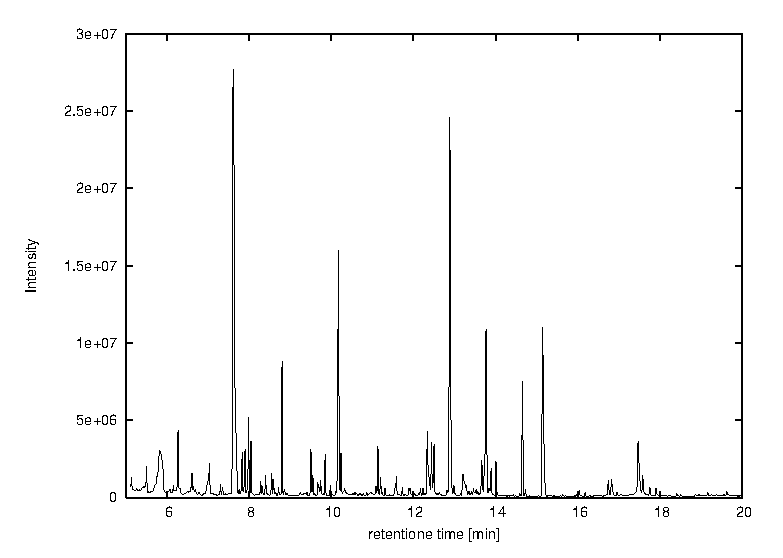
\includegraphics{graphics/tic.eps}
\caption{The Gnuplot plot of the file 'tic.dat'}
\label{tic-plot}
\end{center}
\end{figure}

The method {\tt get\_intensity\_matrix()} of ChemStation object returns
the entire matrix of intensities:

\begin{verbatim}
>>> im = andi_data.get_intensity_matrix()
>>> print "Dimensions of the intensity matrix are:",len(im),"x",len(im[0])
Dimensions of the intensity matrix are: 2784 x 501
\end{verbatim}

\noindent
This data matrix contains 2784 time points (MS scans), and each time point
corresponds to a mass spectrum of 501 m/z points.

The intensity matrix can be saved to a file with the function 'save\_data()':

\begin{verbatim}
save_data("output/im.dat", im)
\end{verbatim}

The entire data (ie. ChemStation object) can be saved as CSV with the method
{\tt export\_csv()}. For example,

\begin{verbatim}
>>> andi_data.export_csv("output/data")
\end{verbatim}

\noindent
will create 'data.im.csv, data.mz.csv, and data.rt.csv where these are the
intensity matrix, retention time vector, and m/z vector in the CSV format.

\section{Example 2: Creating signal peaks}

\noindent
{\em This example is in pyms-test/02}
G
In PyMS a signal peak is represented as 'Peak' object defined in
pyms.Peak.Class.py. A peak object is initialized with two arguments:
peak retention time and peak raw area. The following commands create
a peak named 'p' with the retetion time of 5.553 min and a peak area
of 2759280 (this is the peak no. 3 in the ChemStation peak area report
file 'a0806\_140.txt'):

\begin{verbatim}
>>> from pyms.Peak.Class import Peak
>>> p = Peak(5.553*60.0,2759280)
\end{verbatim}

\noindent
As a matter of convention PyMS internally stores retention times in
seconds, hence above the retention time is multiplied by 60. Peak
raw area is in arbitrary units.

Peak properties can be accessed through its attributes:

\begin{verbatim}
>>> print "Peak retention time is", p.rt
Peak retention time is 333.18
>>> print "Peak raw area is", p.raw_area
Peak raw area is 2759280.0
\end{verbatim}

\noindent
Other important properties of a peak object are peak normalized area
and peak mass spectrum. The peak created in the above example does
not have values associated with these two attributes, and they are
merely initialized to 'None':

\begin{verbatim}
>>> print "Peak normalized area is", p.norm_area
Peak normalized area is None
>>> print "Peak mass spectrum is", p.mass_spectrum
Peak mass spectrum is None
\end{verbatim}

\noindent
The peak mass spectrum can be set by calling the method {\tt set\_mass\_spectrum()}.
This method requires the raw data, and fetches mass spectrum at peak
retention time:

\begin{verbatim}
>>> p.set_mass_spectrum(andi_data)
\end{verbatim}

\noindent
This will set the mass spectrum attribute: 

\begin{verbatim}
>>> print p.mass_spectrum
 49976  54520 102752  15570   1872  18392   8765  14966  46136  16141
  1635   1743    686   1019    712   1199   1641   3182   1234  30400
  4261   3746   3348  82392   8354  24824   3797   6086  23312 140480
[--output deleted--]
\end{verbatim}

\noindent
These are m/z channel intensities in arbitrary units. The m/z values
themselves are in the mass list attribute:

\begin{verbatim}
>>> print p.mass_list
[50, 51, 52, 53, 54, 55, 56, 57, 58, 59, 60, 61, 62, 63, 64, 65,
66, 67, 68, 69, 70, 71, 72, 73, 74, 75, 76, 77, 78, 79, 80, 81,
[--outout deleted--]
\end{verbatim}

\noindent
The length of the two arrays must match:

\begin{verbatim}
>>> print len(p.mass_spectrum)
501
>>> print len(p.mass_list)
501
\end{verbatim}

The mass spectrum can be written to a file by calling the peak
{\tt write\_mass\_spectum()} method:

\begin{verbatim}
>>> p.write_mass_spectrum("output/ms.dat")
\end{verbatim}

\noindent
The file 'output/ms.dat' contains the pairs (mz, intensity), one pair
per line:

\begin{verbatim}
$ head output/ms.dat
  50.000        49976.000
  51.000        54520.000
  52.000       102752.000
  53.000        15570.000
  54.000         1872.000
  55.000        18392.000
  56.000         8765.000
  57.000        14966.000
  58.000        46136.000
  59.000        16141.000
\end{verbatim}

\noindent


Figure \ref{mass-spectrum} shows the plot of ms.dat created with the
program Gnuplot. The gnuplot script used to create this plot is
provided as pyms-test/02/output/plot.gnu.

\begin{figure}[htp]
\begin{center}
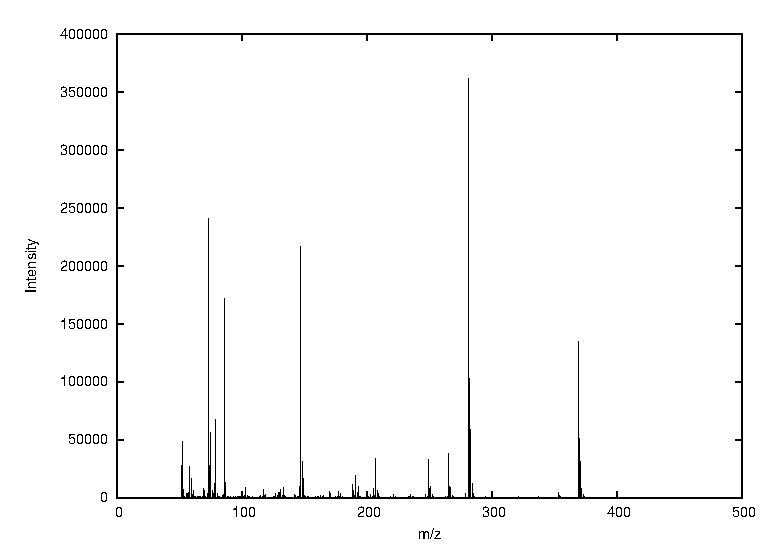
\includegraphics{graphics/ms.eps}
\caption{The plot of the file 'ms.dat' produced with Gnuplot}
\label{mass-spectrum}
\end{center}
\end{figure}

\section{Example 3: Creating an experiment from ChemStation data}

\noindent
{\em This example is in pyms-test/03}

The input files used in this example are 'a0806\_140.CDF' (ANDI-MS data
file exported from Agilent ChemStation) and 'a0806\_140.txt.anno' (the 
corresponding peak area report file generated by ChemStation).

The original peak area report file exported from ChemStation is
'a0806\_140.txt'. This file was manually edited to flag non-informative
peaks, and also peaks which originate from internal reference compounds
added during the sample preparation. For example, below is the snippet
of the original file 'a0806\_140.txt':

\begin{verbatim}
 52   8.215   470  478  480 PV 3   91906   1414873   0.14%   0.056%
 53   8.242   480  483  486 VV 4   99010   1301807   0.13%   0.051%
 54   8.285   486  490  495 VV 2  124626   2241940   0.22%   0.088%
 55   8.337   495  499  501 VV 2   44820    662145   0.06%   0.026%
 
 56   8.365   501  504  506 VV 2   58181    789953   0.08%   0.031%
 57   8.399   506  510  515 VV    713172   9893695   0.97%   0.389%
 58   8.443   515  518  521 VV 5  143812   2590885   0.25%   0.102%
 59   8.477   521  524  526 VV 4  149127   2438042   0.24%   0.096%
 60   8.548   526  536  558 VV 2 55398426 1025005618 100.00%  40.335%
\end{verbatim}

\noindent
and the same file in the file 'a0806\_140.txt.anno'

\begin{verbatim}
 52   8.215   470  478  480 PV 3   91906   1414873   0.14%   0.056%
 53   8.242   480  483  486 VV 4   99010   1301807   0.13%   0.051% BLANK
 54   8.285   486  490  495 VV 2  124626   2241940   0.22%   0.088%
 55   8.337   495  499  501 VV 2   44820    662145   0.06%   0.026%
 
 56   8.365   501  504  506 VV 2   58181    789953   0.08%   0.031%
 57   8.399   506  510  515 VV    713172   9893695   0.97%   0.389%
 58   8.443   515  518  521 VV 5  143812   2590885   0.25%   0.102%
 59   8.477   521  524  526 VV 4  149127   2438042   0.24%   0.096%
 60   8.548   526  536  558 VV 2 55398426 1025005618 100.00%  40.335% BLANK
\end{verbatim}

\noindent
In the file 'a0806\_140.txt.anno' the keywork 'BLANK' was manually
added to peaks 53 and 60, which are known to originate from the
derivatizing agent use in GC-MS data preparation.  These peaks can 
be excluded from the analysis later.

The peak eluting at 15.590 min originated from scyllo-inositol reference
compound added during sample preparation. In the file 'a0806\_140.txt.anno'
this peak was labelled as follows:

\begin{verbatim}
178  15.590  1758 1767 1773 VV   5307268  80504143   7.85%   3.168% RF-SI
\end{verbatim}

\noindent
There could be an arbitrary number of reference peaks in the peak list,
and each must have a unique reference 'tag' starting with 'RF-' and
following with a two letter code denoting a particular reference sompound
(in this case SI for scyllo-inositol).

The ChemStation peak list is loaded in PyMS with the function
'read\_chem\_station\_peaks()':

\begin{verbatim}
>>> from pyms.Peak.List.IO import read_chem_station_peaks
>>> peak_file = "/home/current/proj/PyMS/pyms-data/a0806_140.txt.anno"
>>> peaks = read_chem_station_peaks(peak_file)
 -> Reading ChemStation peak integration report
'/home/current/proj/PyMS/pyms-data/a0806_140.txt.anno'
\end{verbatim}

\noindent
The variable 'peaks' now contains the peaks from the file 'a0806\_140.txt.anno'
This is merely a Python list:

\begin{verbatim}
>>> type(peaks)
<type 'list'>
>>> print "The number of peaks is:", len(peaks)
The number of peaks is: 347
\end{verbatim}

The next step is to set the mass spectrum is set for each peak. For this we need
first to load the raw data:

\begin{verbatim}
>>> import sys
>>> sys.path.append("/home/current/proj/PyMS/")
>>> from pyms.IO.ANDI.Class import ChemStation
>>> andi_file = "/home/current/proj/PyMS/pyms-data/a0806_140.CDF"
>>> andi_data = ChemStation(andi_file)
 -> Processing netCDF file '/home/current/proj/PyMS/pyms-data/a0806_140.CDF'
    [ 3236 scans, masses from 50 to 550 ]
\end{verbatim}

\noindent
The following command sets the mass spectrum for each peak,

\begin{verbatim}
>>> for peak in peaks:
...     peak.set_mass_spectrum(andi_data)
\end{verbatim}

The experiment object is initiated with the list of peaks and the experiment
label, in this case "a0806\_140":

\begin{verbatim}
>>> from pyms.Experiment.Class import Experiment
>>> expr = Experiment("a0806_140", peaks)
\end{verbatim}

\noindent
In the next steps we call a series of methods associated with the experiment
object to set the reference peak, remove blank peaks, create peak normalized
area (in this case the same as peak raw area), purge negative peaks (if
any), and finally select the retention time range for the experiment to
between 6.5 and 21 minutes, discarding all peaks outside this range:

\begin{verbatim}
>>> expr.set_ref_peak("si")
 [ Reference peak found: 'rf-si' @ 935.400 s ]
  [ Removing reference peak 'rf-si' @ 935.400 s ]
>>> expr.remove_blank_peaks()
        [ Designated blank peak at 438.660 s removed ]
        [ Designated blank peak at 494.520 s removed ]
        [ Designated blank peak at 512.880 s removed ]
        [ Designated blank peak at 751.980 s removed ]
>>> expr.raw2norm_area()
>>> expr.purge_peaks()
 Experiment a0806_140: 0 peaks purged (below threshold=0.00)
>>> expr.sele_rt_range(["6.5m", "21m"])
 -> Selecting peaks by retention time (from 6.5m to 21m): 247 peaks selected
\end{verbatim}

Finally, we dump the experiment object to a file allowing it to be used
later, for example in the process of peak alignment (see the example
pyms-test/04):

\begin{verbatim}
>>> from pyms.Experiment.IO import dump_expr
>>> dump_expr(expr, "output/a0806_140.pickle")
 -> Experiment 'a0806_140' saved as 'output/a0806_140.pickle'
\end{verbatim}


